\documentclass[12pt]{article}
\usepackage{amsmath, amssymb}
\usepackage{pdfpages}
\usepackage[a4paper, top=18mm, bottom=18mm, left=10mm, right=10mm]{geometry}
\usepackage[font = normalsize, labelfont = bf]{caption}
\usepackage[font = normalsize, labelfont = bf]{subcaption}
\usepackage{epsf, graphics}
\usepackage[toc,page]{appendix}
\usepackage{tcolorbox}
\usepackage{fancyhdr}
\usepackage{lipsum, lastpage}
\usepackage[official]{eurosym}
\usepackage{colortbl, tabularx}
\usepackage{color, enumerate, natbib}
\usepackage{hyperref}  % this guy must be the last package called
\hypersetup{colorlinks=true, allcolors=blue}


\begin{document}

\pagestyle{fancy}
\lhead{\footnotesize \parbox{11cm}{MHD Workshop Leiden 2021}}
\rhead{\footnotesize \parbox{11cm}{\hfill \textsf{Legolas} demo}}
\renewcommand\headheight{24pt}
\renewcommand\footrulewidth{0.4pt}

\section*{Getting started}
The Legolas code can be found on \href{https://github.com/n-claes/legolas}{GitHub}, installation instructions are on the website. Make sure to look at the prerequisites for both Legolas and Pylbo first before running the code.

\section{Equilibria}
Below is a list of possible setups that can be implemented in the user submodule. We've added a reference figure together with the link to the original work so you can check your implementation and compare with known results.

\subsection{Internal kink modes in force-free magnetic fields}
This setup is taken from \citet{goedbloed2018}, which is a cylindrical equilibrium with a force-free magnetic field of constant $\alpha$ and profiles given by
\begin{equation*}
	\begin{aligned}[t]
		\rho(r) &= \rho_0\left(1 - x^2\right) \\
		v_z(r) &= v_{03}\left(1 - x^2\right) \\
		B_\theta(r) &= J_1(\alpha x) \\
		B_z(r) &= J_0(\alpha x) \\
		T(r) &= \frac{p_0}{\rho(r)}
	\end{aligned}
	\qquad\qquad
	\begin{aligned}[t]
		\rho'(r) &= -\frac{2\rho_0}{a} x \\
		v_z'(r) &= -\frac{2v_{03}}{a} x \\
		B_\theta'(r) &= \frac{\alpha}{2a} \left[J_0(\alpha x) - J_2(\alpha x)\right] \\
		B_z'(r) &= -\frac{\alpha}{a} J_1(\alpha x) \\
		T'(r) &= \frac{2 r p_0}{a^2\rho_0(1 - x^2)^2}
	\end{aligned}
\end{equation*}
where $x = r / a$ and $a$ denotes the outer wall of the cylinder.

\begin{figure}[h]
	\centering
	\begin{minipage}{0.42\textwidth}
		\centering
		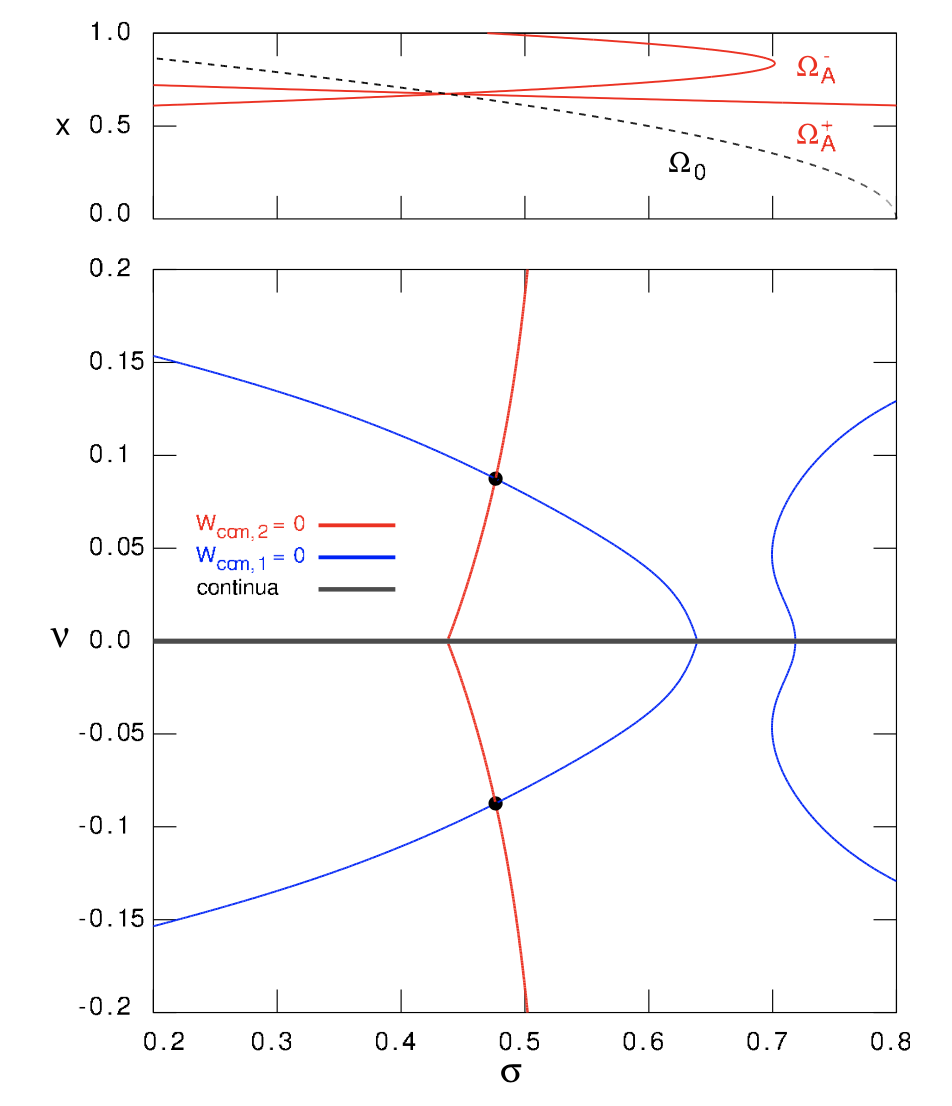
\includegraphics[width=\textwidth]{internal_kink.png}
		\caption{Values $\rho_0 = v_{03} = p_0 = a = m = 1$, $\alpha a = 5$, $k = 0.16\alpha$, incompressible.}
	\end{minipage}\hfill
	\begin{minipage}{0.53\textwidth}
		\centering
		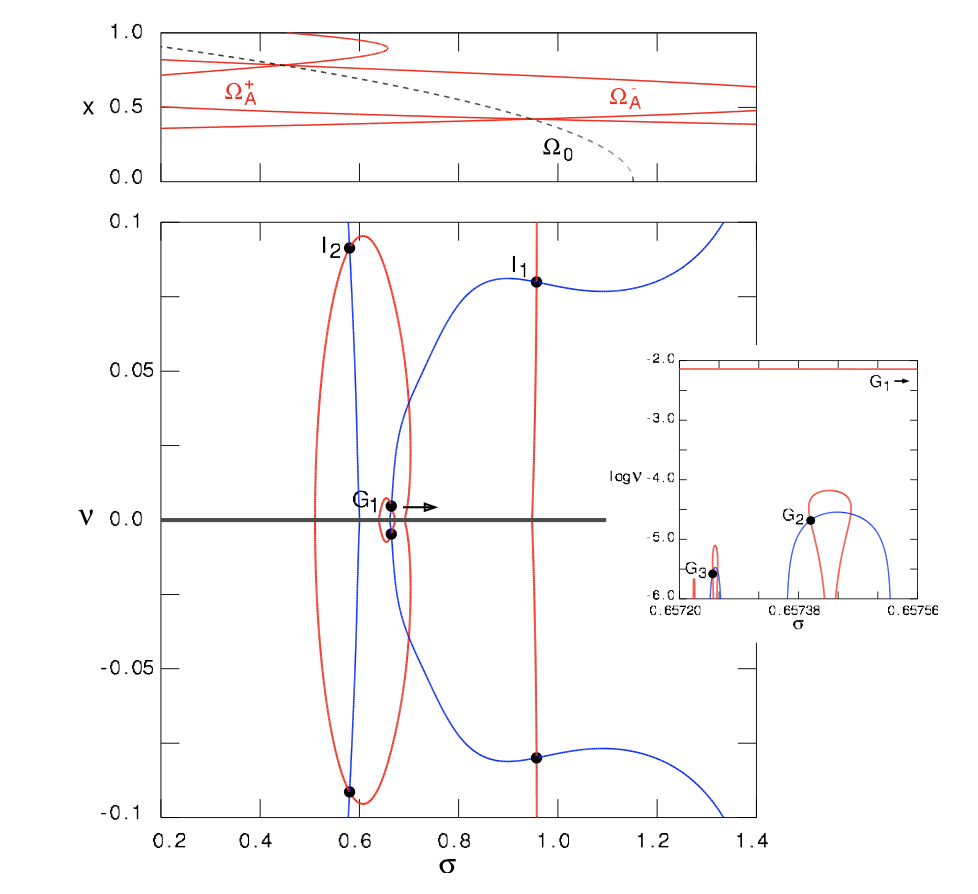
\includegraphics[width=\textwidth]{internal_kink2.png}
		\caption{Values $\rho_0 = p_0 = a = m = 1$, $v_{03} = 0.8$, $\alpha a = 8$, $k = 0.16\alpha$, incompressible.}
	\end{minipage}
\end{figure}


\bibliographystyle{bibstyle}
\bibliography{bibfile}


\end{document}